\chapter{Method} %aj material and method

This chapter presents the setup of the robots and algorithms and the tools utilized. 

%aj 3.1 experiment setup
%3.2 methodology
%3.2.1  autonomous navigation of husky
%3.2.2 autonomous navigation of tb
%3.2.3 mimic algorithm
%3.2.4 platooning

%aj first para(s) should be without section where you explain what is in the chapter. write about the  algorithm (a) imitation/mimic and (b) paltooning

\section{Development tools}
% every  chapter has intro and conclution 
%aj a paragraph explaining what is mentioned in the chapter. write about the building blocks of yuour thesis. please see the teams where i have outlined them. then each section becomes the theory or working principle of the individual components.
This section's purpose is to give an insight into the tools used in this thesis and their working principles. The information here is a collection of what's needed for the experimental setup. For further reading all of the topics here are well documented on the web. 
 
%background /theory should be about - autonomous navigation, slam, collision avoidance, networked communication ... see teams

\subsection{Hardware}

The hardware used in this thesis is presented in Table \ref{tab:HW_list}. Datasheets are linked next to the names.

\begin{table}[H]
    \centering
    \caption{List of hardware used in this thesis.}
    \begin{tabular}{c|c|c}
        Name                    & Reference name    & Short description  \\ \hline
        Clearpant Husky \cite{huskyugv}         & Husky             & Medium sized wheeled robot \\
        Nvidia Xavier 1 \cite{xavierguide}        & Xavier1           & Compact computer controlling the Husky\\
        Ouster OS-1-64 \cite{OS1Datasheet}         & OS1               & 3D LiDAR on the Husky \\
        UM7 Orientation Sensor \cite{um7datasheet} & UM7               & Inertial measurement unit(IMU)  \\
        Husky's wheel encoder   & Wheel encoder     & Measures the movement of the wheels\\
        TurtleBot3 \cite{turtlebot3}          & TB3               & Small sized wheeled robot   \\
        Nvidia Xavier 2         & tb                & Compact computer Controlling TB3  \\
        LDS-01 \cite{lds01}     & LDS-01            & 2D LiDAR on TB3 \\
        OpenCR 1.0 \cite{opencr10}     & OpenCR 1.0        & Microcontroller with IMU for robotics \\
        
    \end{tabular}
    \label{tab:HW_list}
\end{table}

\subsubsection{Xavier}
Xavier or NVIDIA Jetson AGX Xavier Developer Kit is a compact computer for AI applications, with the size 105mm x 105mm x 65mm and the power source being 9 - 20 volts. Its practical for mobile robots. 

The Nividia computers come with their own Linux version, JetPack, based on Ubuntu. The JetPack system includes AI applications. JetPack and the GPU is the reason why the Xavier is suitable for AI applications. The CPU of the Xavier has an ARM architecture. A WiFi module can be attached and is in this project.

\subsubsection{Sensors}

\paragraph{LiDAR}(Laser imaging, Detection, and Ranging) is a method of measuring distances with laser. The principle is sending a laser beam at a target, sensing the reflection, and calculating the distance based on the time between the laser sent and received. 

TurtleBot3 uses a LiDAR called LDS-01, and the Husky uses Ouster OS-1-64. Table \ref{tab:lidar_data} provides relevant data for the LiDAR's. 

\begin{table}[h]
    \centering
    \caption{LiDAR data for LDS-01\cite{lds01} and OS1 \cite{OS1Datasheet}.}
    \begin{tabular}{c|c|c}
        Specifications          & TrutleBot3        & Husky             \\ 
                                & LDS-01            & Ouster OS-1-64    \\ \hline
        Range                   & 120 - 3,500mm     & 0.3m - 120m       \\ \hline
        Vertical resolution     & 1 channel (2D)    & 64 channel (3D)   \\ \hline
        Angular Range           & $360^\circ$       & $360^\circ$       \\ \hline  
        Power source            & Micro USB         & Barrel jack       \\  
                                & 5 volts           & 24 volts          \\ \hline
        Data line               & Micro USB         & Ethernet          \\       
    \end{tabular}
    \label{tab:lidar_data}
\end{table}

\paragraph{Inertial Measurement Unit (IMU)} is an electronic device that uses accelerometers, gyroscopes, and sometimes magnetometers to measure and report a body's specific force, angular rate, and occasionally its orientation.

\paragraph{Rotary encoders} are electro-mechanical devices that measure the position and speed of rotating objects, such as wheels, motors, and joints. Wheel encoders are often used in robotics to estimate position based on kinematics. 

\subsubsection{Husky}
The Husky UGV is a medium-sized Unmanned Ground Vehicle (UGV) from Clearpath. It has fire wheels and a footprint of 990mm x 670mm. It is powered by two 12volts batteries in series, a total of 24 volts. There are three power outputs for external components 5V, 12V, and 24V fused at 5A each. The wheels are controlled by a built-in motor drive with a wheel encoder.

The front and back wheel of each side is mechanically connected, and powered by one motor. Therefore able to turn the Husky's wheels will skid, which makes the turning and odometry inaccurate. 

\subsubsection{TurtleBot3}
The TurtleBot3 Waffle Pi (TB3) is a small robot provided by Open Robotics and ROBOTIS. The footprint of the robot is 138mm x 178mm, it is driven by two front wheels and has two ball casters in the back. Therefore the TB3 has a differential drive, which is a precise way to turn. 

\paragraph{OpenCR1.0} is a multi-purpose board on the TurtleBot3. This board connects to the battery and powers the Xavier and motors for the wheels. The control signal for the wheels comes from the Xavier through the OpenCR1.0 in to the wheels. 
The TurtleBot3 also includes a LiDAR and an IMU on OpenCR1.0 board.

\subsection{Software}

\subsubsection{Ubuntu}

Ubuntu is an open-source operating system(OS) based on Linux\cite{ubuntu}\cite{osi}. It is the most popular Linux distribution and the main OS for ROS2. ROS2 can be used on Windows and Mac as well but is sub optimal. Ubuntu has two main forms desktop and server. The desktop provides a graphical user interface(GUI). Ubuntu server does not have a GUI, and it is just a text-based user interfaces(TUI). The server is more demands less possessing power and storage. 


\paragraph{SSH} or Secure Shell is a network protocol for encrypted communication between two computers on the same network. SSH is a terminal-based program, and therefor there is no GUI just a TUI. 

In robotics, SSH is commonly used. Often it is not practical or possible to connect the robots computer to keyboard and a monitor. A lot of robots have computers running a TUI-based OS, so a monitor would not provide more information than SSH. 

\subsubsection{ROS2} 
 All of the information about Robot operating system 2 (ROS2) has been found on their website\cite{rosfoxydocs}, which is well documented and recommended for further reading. In this section, the necessary concept for the thesis will be briefly presented. 
ROS2 is a meta OS installed on top of another OS. The OS most commonly used is Ubuntu. ROS2 can be described as a base for building robot applications with a set of software libraries and tools. ROS2 is open source and has a large community, this is essential. The large community means that it's a lot of help online. Open source makes it easier to make ROS2 software to different hardware.

A large part of ROS2 is communication with messages. Messages refer to data this can be single variables like "int", "float", "string" and so on. Bigger data types like "Twist.msg" and "Odometry.msg" are also messages, which often contain a hierarchy of data. 
Table \ref{tab:ROS2_topics} shows a list of common ROS/ROS2 topics.
\begin{table}[H]
    \centering
    \caption{Examples of ROS2 topics used in this thesis.}
    \begin{tabular}{c|c}
       Topic name       & Function          \\ \hline
        /cmd\_vel       & Velocity command  \\
        /odom           & Odometer          \\
        /scan           & 2D laser scan     \\
        /points         & 3D laser scan     \\        
        /imu/data       & IMU data          \\
    \end{tabular}
    \label{tab:ROS2_topics}
\end{table}

The standard topic names are convenient but can cause problems when there are multiple types of the same sensor. Namespace solves this problem by putting "/namespace" in front of \topic{/generic\_topic\_name}.  

\paragraph{Nodes} in ROS2 is a lightweight and modular process that performs a specific computation. Each node is identified by a unique name within the ROS2 system. 
ROS2 nodes can be described by what they are commonly used for. 

\begin{itemize}
    \item Publish sensor data: A ROS node can read data from sensors, such as IMU or LiDAR, and publish it to a ROS topic for other nodes to consume, like \topic{/imu/data}, \topic{/scan} or \topic{/points}.
    
    \item Control a robot: A ROS node can send commands to a robot's motors or actuators to control its movement or behavior based on topics like \topic{/cmd\_vel}.
    
    \item Process data: A ROS node can receive data from hardware or other nodes and perform calculations or conversions, such as filtering or mapping for example, a EKF filter node.
    
    \item Provide a user interface: A ROS node can provide a GUI or TUI for users to interact with the system like teleop or Rviz.
    
    \item Manage communication: A ROS node can act as a bridge between different communication protocols or systems, allowing them to exchange data using ROS messages.
    
\end{itemize}

Nodes communicate with each other by publishing messages to topics or subscribing to topics to receive messages. Nodes can also communicate with each other using services which provide a request/response communication pattern. ROS2 nodes can also communicate with each other by using actions, which provide a more complex form of request/response communication pattern that involves feedback and cancellation. Nodes can be started up directly for the terminal or a launch file. 

\paragraph{Launch files} is useful in ROS2 projects where there is often a lot of different hardware that needs to be started or launched to start a complete robot. Python or xml launch files is a script for launching multiple nodes and sending arguments into them. Launch files can also launch other launch files, which is convenient because this is often provided by developers or can be found online. 

\paragraph{ROS arguments} can be passed into nodes and launch files and alter the way they work. What type of arguments is available depends on the function of the node or launch file.  

\iffalse
Arguments can be passed directly into nodes in the terminal like this : 
\begin{lstlisting}[language=bash]
  ros2 run demo_nodes_cpp talker --ros-args -r __ns:=/namespace
\end{lstlisting}
Nodes can also resive arguments in a launch file like this: 
\lstinputlisting[language=Python]{code/talker_launch.py}

For launch files, the argument functions in the same way, just with a bit different syntax. To check if arguments can be passed into a launch file, write --show-args at the end of the launch command, for example: 
\begin{lstlisting}[language=bash]
  ros2 launch turtlebot3_bringup robot.launch.py --show-args
\end{lstlisting}
\fi

\paragraph{Parameter files} is a yaml file with multiple arguments or configurations. Often parameter files can be passed in as an argument.

\paragraph{ROS2 packages} is a standard way to structure ROS2 code, making it essay integrate custom code into ROS2 and share it. A typical ROS2 package contains nodes, launch files, parameter files, and URDF files. Packages are usually available in either source or binary. Source downloads is the raw code of a program and need to be build to run. Binary is a pre build or computer readable. 

\paragraph{URDF} (Unified Robot Description Format) files are used to describe the structure, kinematics, and visual properties of robots. They define the robot's links, joints, sensors, and their relationships. URDF files provide a standardized way to represent robots in a machine-readable format, allowing ROS2 to simulate, visualize, and control them accurately.

\paragraph{tf (Transform)} is a ROS library that handles coordinate frame transformations. It manages the relationships between different frames and enables coordinate conversion for accurate spatial representation in robotics.

\paragraph{rqt} is a visualisation tool for ROS2. It provides a map of nodes and topics on the local network, often used for debugging. 

\paragraph{Gazebo} is a physics-based simulator for testing and developing robotics algorithms. It uses models to represent robots and objects in the simulated environment. Gazebo supports a plugin system for extending its functionality. It provides a GUI for visualizing and interacting with the simulation, which also works great with Rviz.

\paragraph{Rviz} is a 3D visualization tool for ROS2 that allows users to view and interact with robot data in real time. It can display data such as point clouds, laser scans, and 3D models of robots(URDF) and their environments. Rviz allows users to change the perspective of the visualization and interact with the data using mouse and keyboard commands. It can also be used to configure sensors and other components of a robot system by visualizing their data and properties. 

\paragraph{teleop\_twist\_keyboard} or just teleop is a build in tool in ROS2 for controlling robots from the keyboard. It dose this by publishing velocity control from keyboard input on the "/cmd\_vel" topic. Teleop is usually ran on a external laptop for convenience.   

\subsubsection{Navigation} 

\paragraph{Nav2} (Navigation Stack 2) \cite{rosnavigation} is a open-source software framework for autonomous robot navigation in ROS2. It provides a set of reusable and configurable software components for creating navigation systems with path planning, localization, obstacle avoidance, and mapping. Nav2 is built on top of the ROS2 middleware and leverages other ROS2 for communication, hardware integration, simulation, and visualization, such as Gazebo and Rviz. Nav2 is designed to be modular and extensible, allowing developers to customize it to meet the specific requirements of their robots and environments.
Nav2 includes an API(application programming interface)\cite{rosnavAPI}, a set of commands for interacting with Nav2 from Python. Examples of commands can be sending a goal, receive a position and checking if a task (route) is complete.  

To achieve autonomous navigation in this project Nav2 is used in combination with LiDAR, wheel encoders, IMUs and the estimated odometry. 

\paragraph{Odometry} is the use of data from sensors on a mobile robot to estimate its motion, specifically its position and orientation changes over time. Wheel encoders and Inertial Measurement Units (IMUs) are two commonly used sensors. Estimates from wheel encoders struggle with various sources of error, such as slippage, uneven terrain, and imperfect sensors. These errors can accumulate over time and result in significant deviations from the actual position and orientation of the robot[]. Although IMUs are useful for providing real-time data on a robot's motion, they are also subject to various sources of error that can affect their accuracy, such as bias, noise, drift, and temperature changes[]. 
To solve the problems with wheel encoders and IMUs, a common approach is to use sensor fusion techniques, which combine data from multiple sensors to obtain a more accurate estimate of the robot's position and orientation. One common method for sensor fusion is the Extended Kalman Filter (EKF). 

\paragraph{EKF} (Extended Kalman Filter) is a type of recursive Bayesian filter commonly used in control systems for estimating the state of a system with noisy sensor measurements. By combining multiple sensors, a better total estimate can be produced. The EKF is widely used in robotics applications, such as localization and mapping, where it can estimate the position and orientation of a robot based on sensor data, such as GPS, IMU, or wheel odometry.


\section{Experiment setup}
In this section, the setup of Husky and TB3, both hardware and software, will be explained. Further, the setup 
for independently autonomous driving, and at last, the algorithms will be explained. 

% Then how both were setup to drive autonomous independently, lastly the algorithms will be explained. 

%aj remove. good for handover LM its here bc i refrence them later
Before getting into the setup of Husky and TB3 it is necessary to explain the Git repositories made for this project $masteruia$ \cite{masteruia} and $uia\_husky\_0776$ \cite{uiahusky}. 

There were three projects on the Husky at the same time, so a common GitHub was made $uia\_husky\_0776$. All the software used by the Husky in this project is launched from the $uia\_husky\_0776$ such as packages for Husky, OS1, UM7, and $pointcloud\_to\_laserscan$.

$masteruia$ is the other GitHub used in the project and contains two packages $uia\_husky\_0776$ and $tb3\_cpp$.
First off the package called $uia\_husky\_0776$ is a copy of the one talked about above. The folder was made when trying to launch the Husky with namespace, this task was not completed. 
The $tb3\_cpp$ is a standard ROS2 CMake package consisting of a launch file for TB3, nodes for Nav2 API, and platooning algorithm. 
                      
%aj suggest to follow the above structure. the content aslo has to be rewritten. mention about UGV, sensors - lidar, IMU, computing platform - xavier 1 . LM i did not get this 
\subsection{Husky}
\subsubsection{Hardware}
This section will describe the setup of the Husky and its components. 

The UM7 IMU was glued to the center of the tray, and connected with a USB to the Xavier. 
In the Husky, there are two Xavier, where only one of them is used in this project, Xavier1. Both of the Xaviers were placed in the tray and secured by a 3D-printed mount screwed to the bottom plate of the tray. The Xaviers lacked USB ports, so both got a USB hub. Xavier1 got connected to the network by WiFi.
The Ouster LiDAR has two components the laser scanner and the power/data brick. The scanner is mounted on top of an aluminum frame in the front for long-distance scanning. The brick is glued to the front wall of the tray, connected to 24 volt barrel jack and Ethernet form the router. 
The router is mounted in the front of the aluminum frame and powered by a 12 volt barrel jack. 
\begin{figure}[H]
  \centering
  \begin{minipage}[b]{0.4\textwidth}
    \includegraphics[width=\textwidth]{Figures/images/husky_irl.jpg}
    \caption{Photo of Husky}
    \label{fig:husky_irl}
  \end{minipage}
  \hfill
  \begin{minipage}[b]{0.59\textwidth}
    \includegraphics[width=\textwidth]{Figures/drawio/Husky_HW.drawio.png}
    \caption{Husky hardware map, this dose not include components on the Husky used in other projects}
    \label{fig:Husky_HW}
  \end{minipage}
\end{figure}
%aj font size needs to be increased, its not redable LM donew
\subsubsection{Software}
This section describes the setup of the Husky without Nav2, the "base" setup of the Husky. For less confusion, all \topic{topics} and \node{nodes} are colored-coded in the text and are presented with their ROS2 name.
The Xavier1 on the Husky is running Ubuntu 20.04 Desktop \cite{ubuntu20_04} with ROS2 Foxy \cite{rosfoxyinstall} and Galactic \cite{rosgalacticinstall}, Nav2 binary \cite{rosnavinstall}, Husky Foxy Debian packages \cite{huskyinstall} and $uia\_husky\_0776$ \cite{uiahusky}. When setting up the ROS2 software Rviz and rqt was used to test all components. \newline
    
$uia\_husky\_0776$ launches packages for Husky, OS1, UM7 and $pointcloud\_to\_laserscan$. A launch file was made to launch it all at once, "husky.launch.py" in "uia\_husky\_0776/husky\_group/launch/".

Clearpath provides binary packages for the Husky in ROS2 Foxy. Because of this, the whole project was initially setup with Foxy. However, due to another project requiring Galactic the project ended up using both Galactic and Foxy.

%aj why write about another project? LM relvant for what ROS version im using 
The other project was using a ViperX 300 Robot Arm. This arm was easier set up with Galactic, so the project was converted to Galactic. Foxy and Galactic are similar and didn't cause any issues, except for with the Husky package. Clearpath did not provide binary packages for the Husky in Galactic, only source. These source files did not initially work on the Husky. The student working on pick and place made some changes to the source files, making them work. Still, the source files on Galactic are more unstable than Foxy binary's. Therefore the $husky.launch.py$ is launched in Foxy and the rest of the project in Galactic. 

%aj need to understand what you have used
The Husky is launched with the $husky.launch.py$ from $husky\_group$ in the $uia\_husky\_0776$. $husky.launch.py$ pass in parameters and starts $base\_launch.py$, \node{um7\_node}, $os1_launch.py$ and \node{pointcloud\_to\_laserscan}. 

% this should be at the beginning and then eplain this figure in detail
\begin{figure}[H]
    \centering
    \includegraphics[width = 1\textwidth]{Figures/drawio/husky_rqt.drawio.png}
    \caption{This image represents software of the Husky in a rqt format where 
ovals are \node{nodes} and squares is \topic{topics}. This does not include Nav2. The original rqt image can be found here \ref{Appendix:HuskySWmap}. }
    \label{fig:HuskySW}
\end{figure}
% images neeed to be refrenced 

$base\_launch.py$ starts up the /joy\_teleop and /robot\_state system and the nodes \node{/twist\_mux}, \node{/huksy\_velocity\_controller} and \node{/ekf\_node}. 

\begin{itemize}
    \item joy\_teleop system converts a Logitech joystick controllers signal into \topic{joy\_teleop/cmd\_vel} a standard velocity massage with namespace. 
    
    \item \node{/twist\_mux} converts \topic{/cmd\_vel} to \topic{/husky\_velocity\_controller/cmd\_vel\_unstamped} and sends it into \node{/huksy\_velocity\_controller}. Every velocity command for the Husky goes through the \node{/twist\_mux}, joystick, keyboard, and Nav2. 
    
    \item \node{/huksy\_velocity\_controller} controlles the motors and publishes \topic{/odom} based on the wheel encounters on the Husky. 
    
    \item \node{/ekf\_node} fuses odometry(\topic{/odom}) and IMU(\topic{/imu/data}) to \topic{"/odometry/filtered"} to localize the Husky with greater precision[]. 
    
    \item The /robot\_state system combines the URDF with the joint state of the wheels to create an accurate model of the Husky in Rviz. 
    
\end{itemize}

The UM7 ROS2 package where found on GitHub \cite{um7imu}. This package launches a node called \node{/um7\_dirver} publishing data from the IMU on topic \topic{/imu/data}, into \node{/ekf\_node}.
\\ \newline
Ouster has a well-documented GitHub \cite{ousterros} with ROS2 drivers for their hardware, including the OS1. The package starts up a node called \node{/ouster\_driver} which publishes \topic{/points}. 
Since Nav2 uses \topic{/scan} as perception topic, a package called "pointcloud\_to\_laserscan" was installed to make the OS1 communicate with Nav2. "pointcloud\_to\_laserscan" was also found on GitHub \cite{pcl2laser}. 
To be able to use the LiDAR it needs a tf to the Husky. Therefore a custom URDF called "husky\_urdf\_extras.urdf" was made for placing the LiDAR relative to the Husky and visualization LiDAR with its aluminum profile mount. The visualization is based on an STL file which can be found in husky\_group/meshes.
"husky\_urdf\_extras.urdf" is launched together with the standard Husky URDF in "husky.launch.py".  


%aj use simple present. also write what you have done. All the failed attempt goes to discussion
\subsection{TurtleBot3}
\subsubsection{Hardware}
The TurtleBot3 started with no battery and was driven by a Raspberry Pi. The Pi was running Ubuntu Server and had an old student project saved. It had performance issues, and writing in the TUI was choppy. The Pi was flashed with Ubuntu Server 20.04 in an attempt to increase performance. This did not work, so it was decided to switch out the Pi. A Xavier was available, and it is the same as the Husky is using and was therefore chosen. The TurtleBot3 uses a battery similar to RC Cars, RC battery's was ordered though a local hobby store. Figure \ref{fig:TB3HW} shows the map of the TB3 hardware. 

\begin{figure}[H]
  \centering
  \begin{minipage}[b]{0.4\textwidth}
    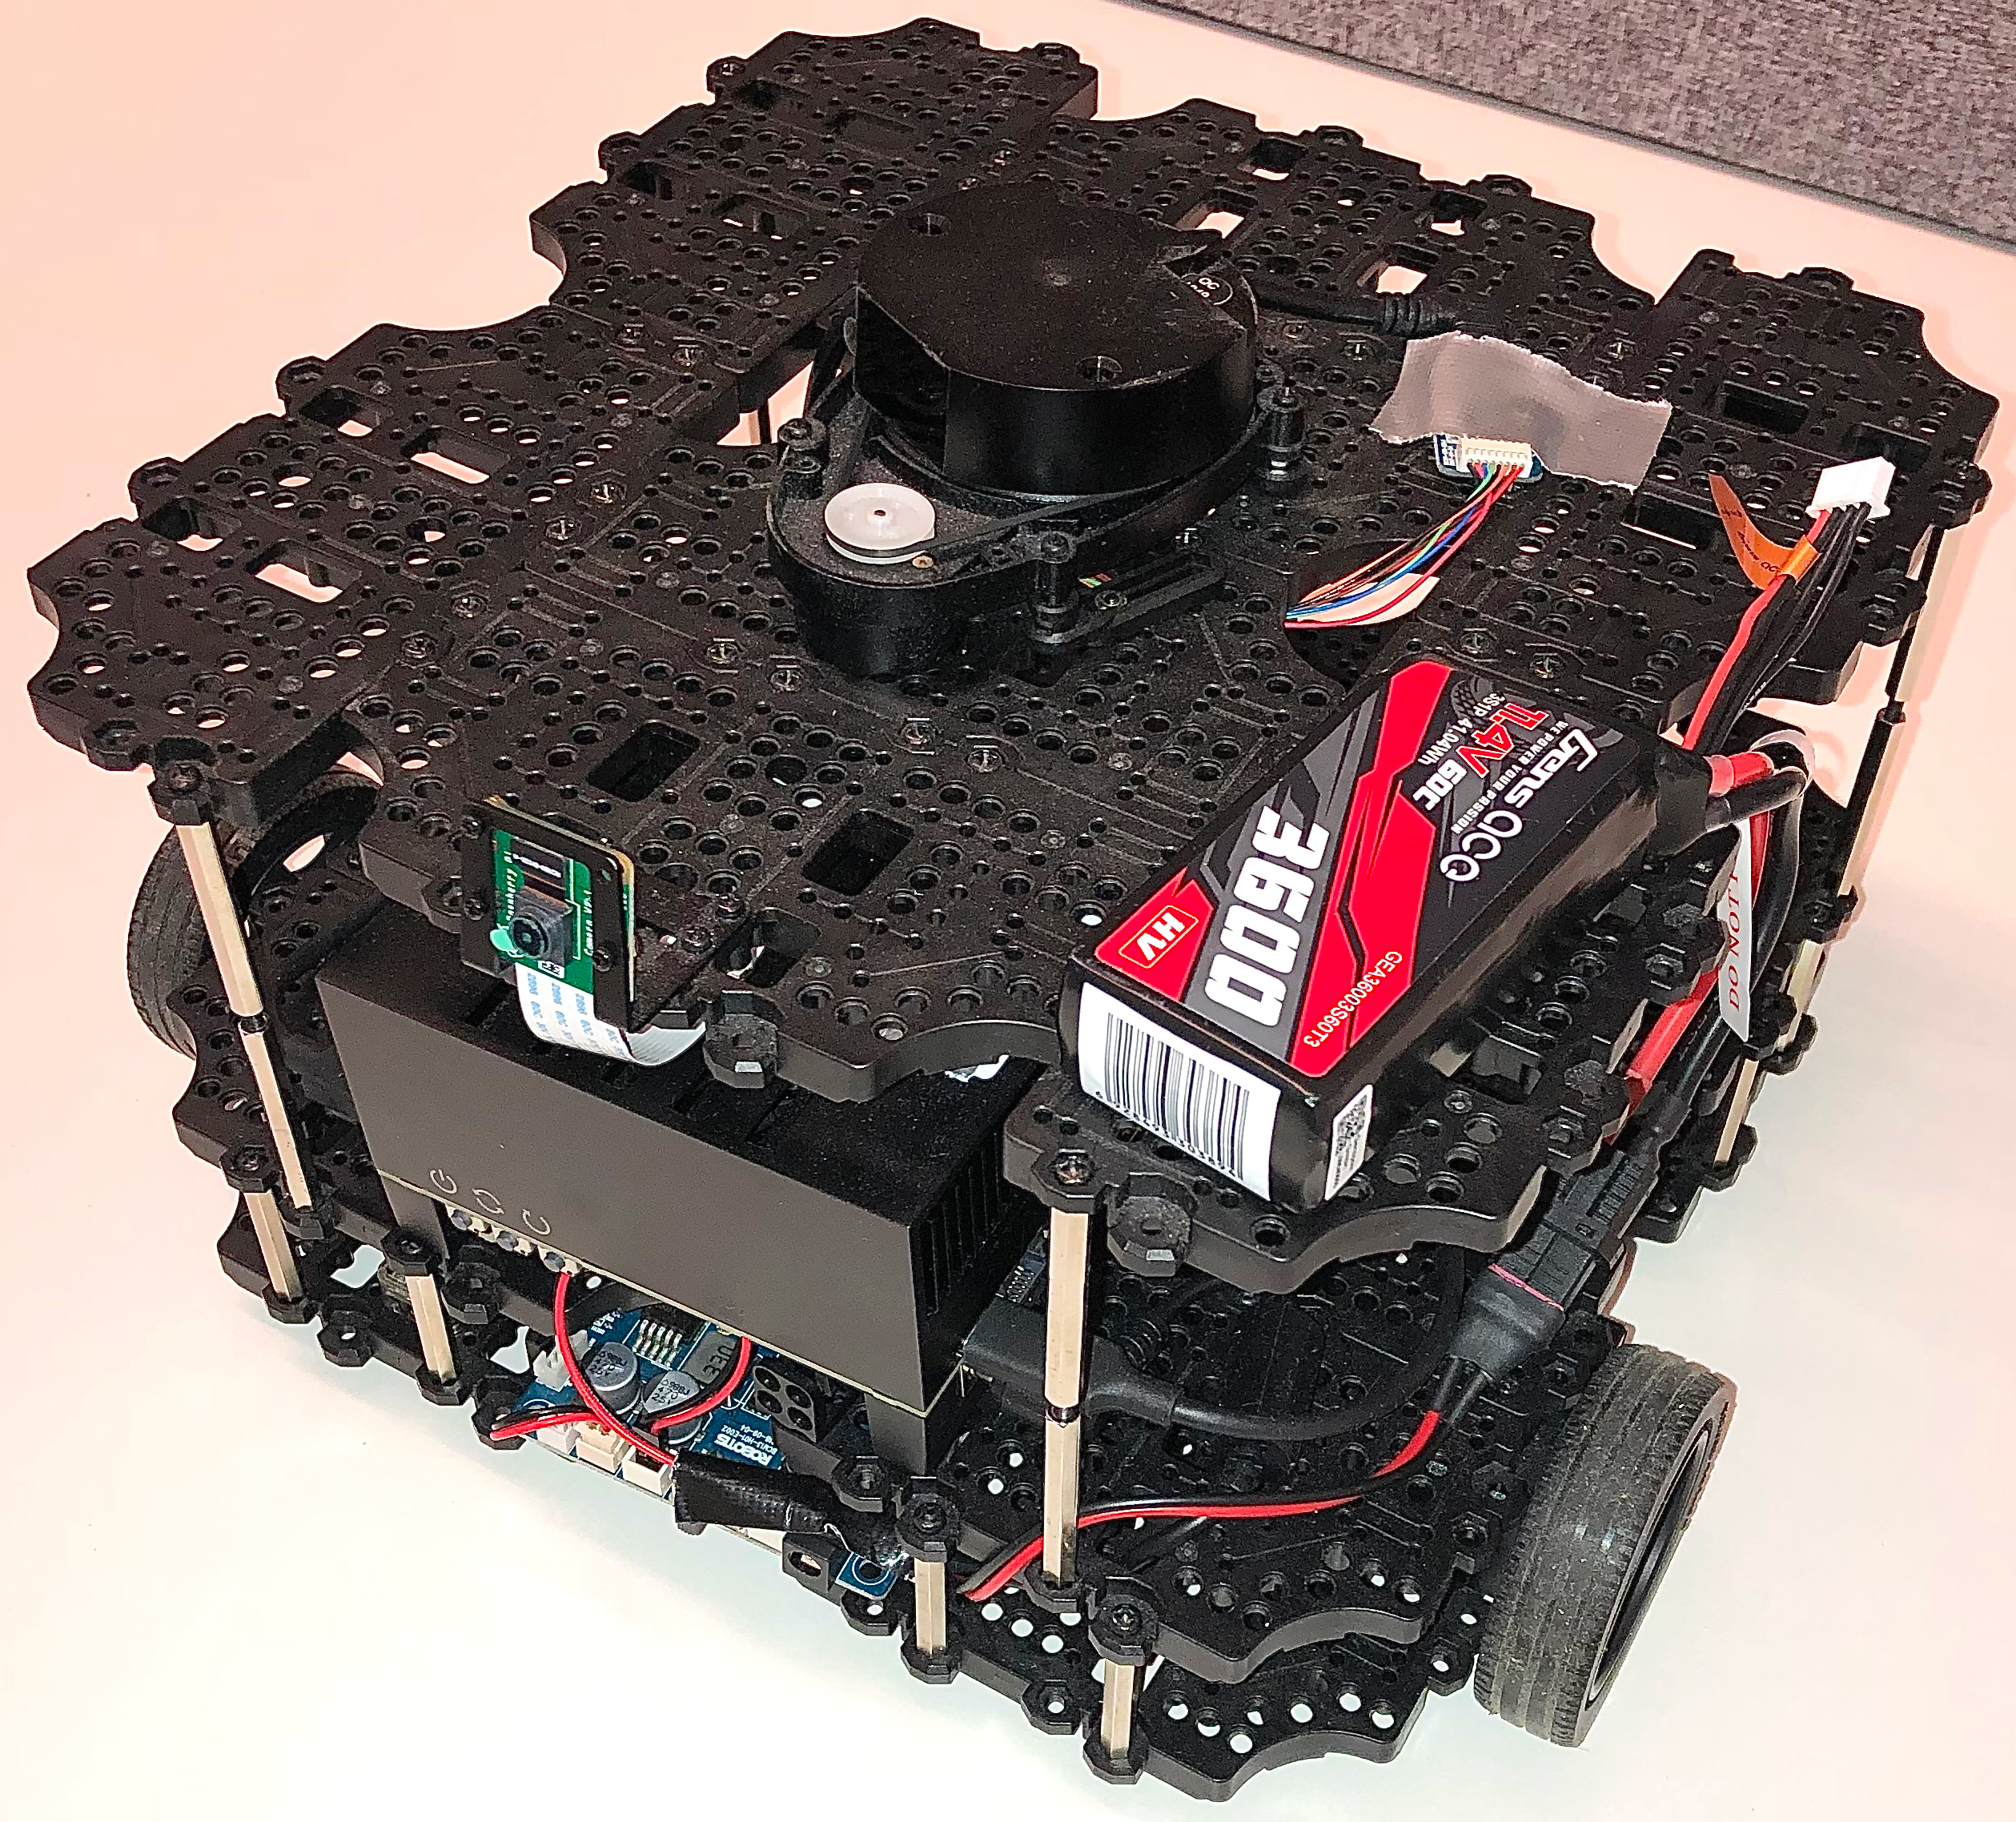
\includegraphics[width=\textwidth]{Figures/images/TB3_irl.png}
    \caption{Photo of TB3}
    \label{fig:TB3_irl}
  \end{minipage}
  \hfill
  \begin{minipage}[b]{0.59\textwidth}
    \includegraphics[width=\textwidth]{Figures/drawio/TB3_HW.drawio.png}
    \caption{TurtleBot3 hardware map}
    \label{fig:TB3HW}
  \end{minipage}
\end{figure}


%aj need to discuss to understand better. I guess fig 3.6 and 3.7 should be demonstrated first and explain them.
\subsubsection{Software}

This will describe the setup of the TB3 without Nav2, the "base" setup TB3.  
The name of the user on the TB3 Xavier is tb and will be the reference. tb is running Ubuntu 20.04 Desktop \cite{ubuntu20_04} with ROS2 Galactic Debian(binary) \cite{rosgalacticinstall}, TB3 packages binary \cite{turtlebot3galactic}, Nav2 binary \cite{rosnavinstall} and $masteruia$ \cite{masteruia}. For less confusion, all \topic{topics} and \node{nodes} have colors and their ROS2 name.

The "robot.launch.py" from the TB3 packages is the file used for launching the TB3 in this project. "robot.launch.py" bring up four nodes \node{/turtlebot3\_node}, \node{/hlds\_laser\_publisher}, \node{/robot\_state\_publisher} and \node{/diff\_drive\_controller}. 
\node{/hlds\_laser\_publisher} starts up LDS1.0 and publishes the LiDAR data on the \topic{/scan} topic. \node{/turtlebot3\_node} publishes five topics and subscribes to one. It subscribes to \topic{/cmd\_vel} converts it to wheel position, and publishes \topic{/joint\_states}. The raw IMU data is picked up by the \node{turtlebot3\_node} and published on the ROS network under \topic{/imu} topic. \topic{/magnetic\_field}, \topic{sensor\_state} and \topic{/battery\_state} are not used in this project. 
\node{/diff\_drive\_controller} fuses \topic{/imu} and \topic{/joint\_states} and publish the fused odometry under \topic{/odom}. 
\node{/robot\_state\_publisher} combines the URDF and \topic{/joint\_states} for a complete description of the TB3 under \topic{/robot\_description}.

\begin{figure}[H]
    \centering
    \includegraphics[width = 1\textwidth]{Figures/drawio/TB3_rqt.drawio.png}
    \caption{TurtleBot3 software map}
    \label{fig:TB3SW}
\end{figure}
\begin{figure}[H]
    \centering
    \includegraphics[width = 1\textwidth]{Figures/drawio/TB3_ns_rqt.drawio.png}
    \caption{TurtleBot3 with namespace software map}
    \label{fig:TB3nsSW}
\end{figure}

\label{method::tb3_cpp_pkg_explained}To achieve namespace like in Figure \ref{fig:TB3nsSW} $tb3\_cpp$ package was made in the $masteruia$ GitHub \cite{masteruia}. This contains three folders launch, params, and src. In launch, the "tb3\_launch.py" is the only one used. The rest is leftovers from working. "tb3\_launch.py" is a launch file for TB3 based on the "robot.launch.py" from "turtlebot3\_bringup". Here is how it works in order: 
\begin{enumerate}
\item Exporting "TURTLEBOT3\_MODEL" is required by "robot.launch.py" 
\item Opens access to LiDAR and OpenCR1.0 
\item Pushing namespace to TB3 
\item Finding and executing standard TB3 launch
\item Passing in custom parameters file to add namespace to all the nodes 
\end{enumerate}  

The $params$ folder is full of work leftovers except for $tb3\_param.yaml$, witch is a copy of the standard TB3 waffle parameter file with "tb:" added in front of the nodes for namespacing.

Last folder $src$ contains nodes from this project. $cmd\_vel\_subpub\_v1.py is the algorithm Time Delay \ref{Platooning_algorithm}. $feedback.py$, $nav2.py$, $pose\_pub\_v*.py$ and $pose\_sub\_v*.py$ is nodes used when attempting to use Nav2 API for a platooning algorithm \ref{Further_work_Nav2_API}.

%aj algorithm required or flowchart here. The implementation explained can be moved to appendix 
\subsection{Autonomous driving on Husky and TB3 independently} \label{Autonomous driving on Husky and TB3 independently}
% Both robots were set up to drive autonomously independently and are able to do it . In the beginning, it was thought that this was necessary to archive autonomous platooning. There were two ways the robots could drive autonomously with and without a pre-made map. 
The two robots were set up to drive autonomously independently and could do so. This was the initial setup. However, not essentially necessary for both robots, only the Husky. There are two ways the robots can drive autonomously, with or without a pre-made map.

Driving with simultaneous localization and mapping (SLAM) and navigation or without a pre-made map. First, the base of the robot is launched, then SLAM lastly, navigation. There are multiple ways of launching SLAM: 
\begin{lstlisting}[language=bash]
    ros2 launch slam_toolbox lifelong_launch.py 
    ros2 launch slam_toolbox online_async_launch.py
    ros2 launch slam_toolbox online_sync_launch.py
\end{lstlisting}
Read more about SLAM here \cite{slamtoolboxgithub}. All of the methods worked but "online\_async" was the most consistent and, therefor used. 

Here is how the Husky was launched to SLAM and navigate: 
Terminal 1:
\begin{lstlisting}[language=bash]
    source /opt/ros/foxy/setup.bash
    source uia_husky_0776/install/local_setup.bash
    ros2 launch husky_group husky.launch.py
\end{lstlisting}
Terminal 2, note "use\_sim\_time:=false because" its not a simulation:
\begin{lstlisting}[language=bash]
    source /opt/ros/galactic/setup.bash
    ros2 launch slam_toolbox online_async_launch.py use_sim_time:=false
\end{lstlisting}
Terminal 3, note custom parameter file:
\begin{lstlisting}[language=bash]
    source /opt/ros/galacitc/setup.bash
    ros2 launch nav2_bringup navigation_launch.py params_file:=uia_husky_0776/husky_group/params/nav2_params.yaml
\end{lstlisting}

The launch setup for the TB3 for SLAM and navigating at the same time: 
Terminal 1, note the "PushRosNamespace" where commented out in launch before this: 
\begin{lstlisting}[language=bash]
    source /opt/ros/galactic/setup.bash
    source masteruia/tb_ws/install/setup.bash
    ros2 launch tb3_cpp tb3_launch.py
\end{lstlisting}
Terminal 2, note "use\_sim\_time:=false because" it is not a simulation:
\begin{lstlisting}[language=bash]
    source /opt/ros/galactic/setup.bash
    ros2 launch slam_toolbox online_async_launch.py use_sim_time:=false
\end{lstlisting}
Terminal 3: 
\begin{lstlisting}[language=bash]
    source /opt/ros/galacitc/setup.bash
    ros2 launch nav2_bringup navigation_launch.py 
\end{lstlisting}

Navigating with a pre-made map uses the same setup for the robots, but SLAM is not launched and the localization\_launch.py is used inserted of navigation\_launch.py. The map is passed into localization\_launch.py as an argument. The map can be made using SLAM with navigation or teleop. 

% basically you are doing (a) mimic and (b) platooning. so keep section name -algorithm and sub section / paragraph as mimic and platooning
\subsection{Platooning algorithm} \label{Platooning_algorithm}

Multiple methods of the algorithm have been explored, "Mimic", "Time delay", "Nav2 API" and "AprilTags/ArUco". The first two were completed and tested in the real world. "Nav2 API" started on and not finished, and "AprilTags/ArUco" were just researched. These are discussed in Further work \ref{Further work}. 

%aj algorithm required or flowchart here. The implementation explained can be moved to appendix 
\paragraph{Mimic} \label{Mimic} is a method where two robots copy each other despite different hardware. The Husky and TB3 receive the same \topic{/cmd\_vel} from either teleop or Nav2 running on the Husky. In the Husky and TB3 software, this velocity command is converted to wheel movement.  

\begin{figure}[H]
    \centering
    \includegraphics[width = 0.5\textwidth]{Figures/drawio/FlowChart_Mimic.drawio.png}
    \caption{Flow chart Mimic algorithm}
    \label{fig:FlowMimic}
\end{figure}

Mimic is set up with launching the Husky and the TB3 without namespace. If launched correctly, they should both subscribe to the \topic{/cmd\_vel}. The source for the \topic{cmd\_vel} can be teleop or Nav2. Launching Nav2 is described here \ref{Autonomous driving on Husky and TB3 independently}. 

%%aj algorithm required or flowchart here. The implementation explained can be moved to appendix. rename platooning
% aj you are mixing method with implementation. What you describe here is implementation. need to discuss how this can be rewritten.
\paragraph{Time delay} \label{Time delay} is method of platooning. It is based on a node called \node{subpub}, which subscribes to the \topic{/cmd\_vel} and saves it in an array. The array has a length of 9 and can be adjusted. The publisher will publish the value one in front of the last saved value, so the publisher is one array behind the subscriber creating the time delay. 
%aj you are again mixing ros implementation and method. We keep  it as it is now as we do not have time to changes. This could be well written. 
\begin{figure}[H]
    \centering
    \includegraphics[width = 0.8\textwidth]{Figures/drawio/Time_delay_pricipal.drawio.png}
    \caption{Principal behind the Time delay algorithm}
    \label{fig:TimeDelayPrincipal}
\end{figure}

The node \node{subpub} is launched with a file called $cmd\_vel\_subpub\_v1.py$ from the $tb\_cpp$ package\ref{method::tb3_cpp_pkg_explained}. Has three main components a subscriber, publisher, and array. 

When $cmd\_vel\_subpub\_v1.py$ is started, it sets initial \py{self.i}, \py{self.delay}, \py{self.submsg}, \py{self.array\_linear\_x} and \py{self.array\_angular\_z}. \py{self.i} is counter for the array and will increase as the \node{subpub} node loops. The counter determines the position of the array the subscriber saves values and the. \py{self.delay} is the length of the array. Twist() is a ROS data type for velocity commands witch the \py{self.submsg} is initialized with, because it is going to receive velocity commands from \topic{/cmd\_vel}. \py{self.array\_linear\_x} is initialized with velocity command for compensating for the TB3 starting one meter behind the Husky. \py{self.array\_angular\_z} is initialised with zero because the TB3 start directly behind the Husky with no angle.

The subscriber saves the \topic{/cmd\_vel} to \py{self.submsg} every 0.5 seconds. 

The publisher initializes \py{pubmsg} with an empty Twist() structure to ensure the correct data type and resetting of old values. Then \py{self.array\_linear\_x} and \py{self.array\_angular\_z}are saved into the \py{pubmsg}. After these values are stored in \py{pubsmg} new ones from \py{slef.submsg} are loaded in. This is the reason the publisher is one array behind the subscriber. The counter is then increased by one. Lastly, the \py{self.submsg} and \py{pubmsg} are printed and published under \topic{/tb/cmd\_vel}. An if statement is added so the array will loop. The publisher loops every 0.5 seconds like the subscriber. 

 \begin{lstlisting}[language=Python, caption=Platooning algortihem Time Delay]
#!/usr/bin/env python3
import rclpy 
from geometry_msgs.msg import Twist 
from rclpy.node import Node
import time 

# converts cmd_vel to tb/cmd_vel with a time delay

class subpub(Node):
    def __init__(self):
        super().__init__('subpub')
        self.subscription = self.create_subscription(Twist, 'cmd_vel', self.listener_callback, 10)
        self.subscription
        self.publisher_ = self.create_publisher(Twist, 'tb/cmd_vel', 10)
        self.timer = self.create_timer(0.5, self.timer_callback)
        self.i = 0
        self.delay = 9
        self.submsg = Twist()  # Initialize the submsg attribute to Twist() 
        self.array_linear_x = [0.25] * self.delay #set initial vel start here 
        self.array_angular_z = [0.0] * self.delay

    def listener_callback(self,submsg):
        self.submsg = submsg

    def timer_callback(self):
        pubmsg = Twist()

        pubmsg.linear.x = self.array_linear_x[self.i] 
        pubmsg.angular.z = self.array_angular_z[self.i]
        
        self.array_linear_x[self.i] = self.submsg.linear.x
        self.array_angular_z[self.i] = self.submsg.angular.z
        
        self.i = self.i + 1 

        print('sub = ', self.submsg, '\n')
        print('pub = ', pubmsg, '\n')
        self.publisher_.publish(pubmsg)
        if self.i == self.delay :
            self.i = 0

def main(): 
    rclpy.init()
    publisher = subpub()  
    rclpy.spin(publisher)   
            
    rclpy.shutdown()

if __name__ == '__main__' : 
    main()          
\end{lstlisting}

\iffalse
\begin{figure}[H]
    \centering
    \includegraphics[width = 0.8\textwidth]{Figures/drawio/cmd_vel_subpub.png}
    \caption{Flow chart Time delay algorithm}
    \label{fig:TimeDelayFlow}
\end{figure}
\fi
%increase font size for better readiblity. explain this flow chart comprehensively

Time Delay is set up by launching the Husky and the TB3 with the namespace /tb. Then teleop on an external computer is launched, or Nav2 on the Husky is launched \ref{Autonomous driving on Husky and TB3 independently}. Since the TB3 starts behind the Husky, this needs to be compensated for. Therefore the Delay Array has initial velocity, which makes the TB3 move one meter forward. As a result, the center of the TB3 needs to be placed one meter behind the Husky's center when the robots are lined up the start the node \node{subpub}. Because of the initial velocity of the TB3 the Husky needs to be driven forward right after starting \node{subpub}, or they will collide. This algorithm where tested, filmed, and discussed here \ref{HuskyNav2 TBsubpub}. 